%% --------------------------------------------------------------
%%
%% T H E O R Y
%%
%% --------------------------------------------------------------



\section{Phsyics}
\subsection{Dynamics}
\begin{frame}{}  %% ---------- Intro/motivation 
    \begin{tikzpicture}[overlay,remember picture]
        \uncover<1->{ % <-> |
            \node (t1) [anchor=center,scale=1,opacity=1] at ([shift={(-3.5cm,-0.5cm)}]current page.center){
                \parbox{0.6\textwidth}{
                    Blast wave dynamics under ``thin-shell'' approximation. 
                    \begin{itemize}
                        \item jet/ejection duration is short (ejecta thickness is small)
                        \item $E_{\rm kin} \gg e_{\rm th}, P$
                        \item $4$ region system 
                    \end{itemize}
                    \begin{equation*}
                        E = \Gamma M_{0} c^2 + T^{00}V, \hspace{2mm}
                        T^{00} = (\epsilon' + P')\Gamma - P'
                    \end{equation*}
                    \begin{equation*}
                        P' = (4/3)(\Gamma^2-1)\rho c^2, \hspace{2mm}
                        \rho' = 4\Gamma\rho, \hspace{2mm}
                        \epsilon' = 4\Gamma\rho c^2
                    \end{equation*}
                    After $dt$, blast-wave sweeps up $dm$ 
                    from ISM, and energy conservation gives $d\Gamma$.
                    Separate inclusion of $d\theta/dt$. 
            }};
        }
        \uncover<1->{ % <-> |
            \node (t1) [anchor=center,scale=1,opacity=1] at ([shift={(4.2cm,-2.0cm)}]current page.center){
                \parbox{0.5\textwidth}{
                    \textbf{Shock downstream}: \\
                    \begin{itemize}
                        \item fluid compression;
                        \item magnetic field amplification ($\varepsilon_B$)
                        \item first order Fermi acceleration ($\varepsilon_e$)
                    \end{itemize}
            }};
        }
        \uncover<1-1>{ % <-> |
            \node (img1) [anchor=center,scale=1,opacity=1] at ([shift={(4.0cm,2.0cm)}]current page.center){
                \parbox{0.5\textwidth}{
                    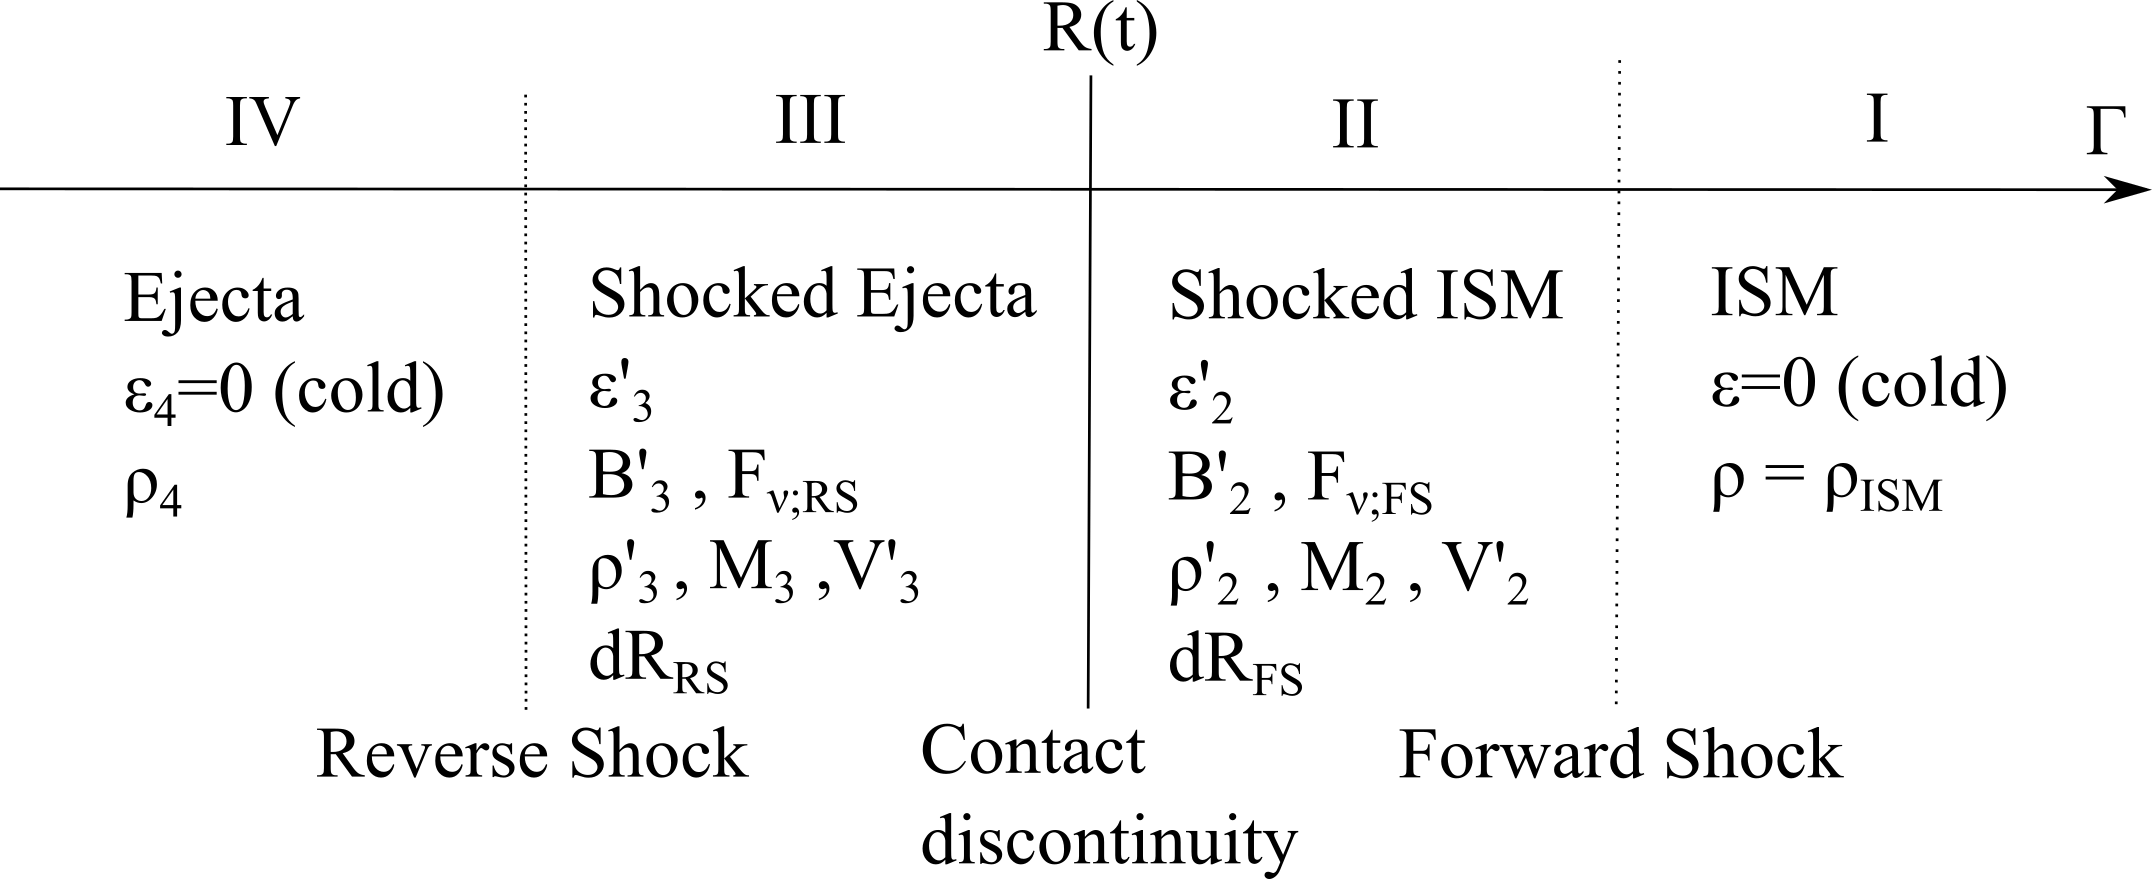
\includegraphics[height=3.0cm]{figures/blast_wave_struct.png}
            }};
        }
    \end{tikzpicture}
\end{frame}


% =============================================================================================

\subsection{Electron distribution in shock downstream}
\begin{frame}{}  %% ---------- Intro/motivation 
    \begin{tikzpicture}[overlay,remember picture]
        \uncover<1->{ % <-> |
            \node (t1) [anchor=center,scale=1,opacity=1] at ([shift={(-3.8cm,-0.2cm)}]current page.center){
                \parbox{0.5\textwidth}{
                    % power = energy/time/steradian/frequency
                    Fokker-Plank type equation:
                    %                    \begin{equation*}
                        %                        \frac{\partial}{\partial t}n_e(\gamma_e,t) = \frac{\partial}{\partial \gamma_e} \Bigg( -\frac{\sigma_T B^2}{6 \pi m_e c} \gamma_e^2 \Bigg) n_e(\gamma_e, t) + Q(\gamma)
                        %                    \end{equation*},
                    %                    where $Q(\gamma_e)\propto\gamma_e^{-p}$ with $\gamma_{m}\leq\gamma_e\leq\gamma_{\rm max}$ 
                    %
                    \begin{equation*}
                        \frac{\partial N(\gamma, t')}{\partial t'} = -\frac{\partial}{\partial \gamma}\Big[ \big( \dot{\gamma}_{\rm syn} + \dot{\gamma}_{\rm adi} N(\gamma, t') \big)  \Big] + Q(\gamma, t')
                    \end{equation*}
                    %
                    \begin{equation*}
                        \dot{\gamma}_{\rm syn} = - \frac{4}{3}\frac{\sigma_T c}{m_e c^2}\gamma^2, \hspace{3mm} \dot{\gamma}_{\rm adi} = -\frac{\gamma \beta_e^2}{3}\frac{d\ln V'}{dt'}, 
                    \end{equation*}
                    %
                    \begin{equation*}
                        Q(\gamma,t) = 
                        %                        \frac{dN_{\rm inj}}{dt d\gamma}=
                        \begin{cases}
                            \textcolor{red}{Q_0}(\gamma_m, t)\Big(\frac{\gamma}{\gamma_m}\Big)^{-p} & \gamma\in(\gamma_m,\gamma_M), \\
                            0 & \text{elswhere}.
                        \end{cases}
                    \end{equation*}
                    %
                    Is $Q_0 = f(B)$ -- YES! 
                    
                    Steady state solution $\partial/\partial t' = 0$ and $\dot{\gamma}_{\rm adi} = 0$.
                    Cooling $\gamma_c = 6\pi m_e c / ( \sigma_T B^2 t )$.
                    
                    Electron cooling modifies distribution
            }};
        }
        \uncover<1->{ % <-> |
            \node (t1) [anchor=center,scale=1,opacity=1] at ([shift={(4.5cm,-0.5cm)}]current page.center){
                \parbox{0.45\textwidth}{
                    %
                    %                    \begin{equation*}
                        %                        \gamma_c = \frac{6\pi m_e c}{\sigma_T B^2 t}, 
                        %                    \end{equation*}
                    Electrons $\gamma > \gamma_c$ occupy $(\gamma/\gamma_c)^{-1}\ll 1$ fractional depth. 
                    Effective line-of-sight electron distribution
                    \begin{equation*}
                        \Big\langle \frac{\partial N}{\partial \gamma} \Big\rangle \propto  \frac{\partial N}{\partial \gamma}  \min \Big( 1, \frac{\gamma_c}{\gamma} \Big)
                    \end{equation*}
                    %
                    \begin{equation*}
                        \Big\langle \frac{\partial N}{\partial \gamma} \Big\rangle_{\rm fc} \propto
                        \begin{cases}
                            \gamma^{-p} & \gamma_m < \gamma < \gamma_c; \\
                            \gamma^{-p-1} & \gamma > \gamma_c
                        \end{cases}
                    \end{equation*}
                    %
                    \begin{equation*}
                        \Big\langle \frac{\partial N}{\partial \gamma} \Big\rangle_{\rm sc} \propto
                        \begin{cases}
                            \gamma^2 & \gamma_c < \gamma < \gamma_m; \\
                            \gamma^{-p-1} & \gamma > \gamma_m
                        \end{cases}
                    \end{equation*}
                    %
                    Afterglow spectrum is defined by $\gamma_m$ and $\gamma_c$
            }};
        }
    \end{tikzpicture}
\end{frame}



% =============================================================================================

\subsection{Cyclosynchrotron emission}
\begin{frame}{}  %% ---------- Intro/motivation 
    \begin{tikzpicture}[overlay,remember picture]
        \uncover<1->{ % <-> |
            \node (t1) [anchor=center,scale=1,opacity=1] at ([shift={(-0.0cm,-0.2cm)}]current page.center){
                \parbox{1.1\textwidth}{
                    % power = energy/time/steradian/frequency
                    \begin{equation*}
                        \boldsymbol{\eta}(\boldsymbol{\beta},\theta)d\omega = \frac{e^2 \omega^2}{2 \pi c}\Bigg[ \sum_{m=1}^{\infty} \Bigg( \frac{\cos\theta - \beta_{||}}{\sin \theta} \Bigg)^2 J_m^2(x) + \beta_{\perp}^2 J_m^{'2}(x) \Bigg]\delta(y) d\omega
                    \end{equation*}
                    where $x = (\omega/\omega_0)\beta_{\perp}\sin\theta$
                    $y=m\omega_0 - \omega(1 - \beta_{||}\cos\theta)$,
                    $\delta(y)$ is the delta function $J_m(x)$ is the Bessel function, 
                    $\beta_{||} = \beta\cos\theta_p$, $\beta_{\perp}=\beta\sin\theta_p$, 
                    with $\theta_p=\angle(\boldsymbol{\beta},\boldsymbol{B})$.
                    \begin{itemize}
                        \item Cyclotron, $m\beta \ll 1$: Expand $J(x)$ to lowest $x$, for successive harminics. 
                        \item Synchrotron $\gamma_e \gg 1$ : $J(x)$ approximated by modified Bessel function
                    \end{itemize}
                    \begin{equation*}
                        \frac{dE}{d\omega} = \frac{\sqrt{3}e^3 B \sin\theta_p}{2 \pi m_e c^2}
                        \frac{\omega}{\omega_c}\int_{\omega/\omega_c}^{\infty}F_{5/3}(\xi)d\xi,
                    \end{equation*}
                    where $\omega_c = (3/2) \gamma^2 \omega_b \sin \theta_p$
                    \begin{equation*}
                        L_{\omega} = 
                        %                        \frac{dE}{d\omega}=
                        2\pi\int_0^1 
                        %                        d\beta n(\beta) 
                        \frac{\partial N}{\partial \gamma_e} d\gamma_e
                        \int_0^1 d(\cos\theta_p) \int_{-1}^{1}d(\cos\theta)\boldsymbol{\eta}_{\boldsymbol{\beta},\theta}.
                    \end{equation*}
            }};
        }
        %        
        %        \uncover<1->{ % <-> |
            %            \node (t1) [anchor=center,scale=1,opacity=1] at ([shift={(0.0cm,-3.8cm)}]current page.center){
                %                \parbox{1.1\textwidth}{
                    %                    \red{Questions}: remnant's lifetime; ejecta properties; \rproc{} cites
                    %            }};
            %        }
        
    \end{tikzpicture}
\end{frame}

% =============================================================================================

\subsection{Synchrotron spectrum from non-thermal electrons}
\begin{frame}{}  %% ---------- Intro/motivation 
    \begin{tikzpicture}[overlay,remember picture]
        \uncover<1->{ % <-> |
            \node (t1) [anchor=center,scale=1,opacity=1] at ([shift={(-4.0cm,2.2cm)}]current page.center){
                \parbox{0.55\textwidth}{
                    Consider
                    $dN/d\gamma_e\propto \gamma^{-p}$, with min. $\gamma_m$ and cool. $\gamma_c$. \\
                    Spectrum is determined by the location of $\nu_c = \gamma_c^2 \nu_g$, 
                    $\nu_g=q_e B / (2\pi m_e c)$ is a gyrofrequency. $F_{\nu}=N_e P_{\nu;\rm max}/4\pi D^2$  where $P_{\nu}\approx \Gamma B m_e c^2 \sigma_T / 3q_e$
            }};
        }
        \uncover<1->{ % <-> |
            \node (t1) [anchor=center,scale=1,opacity=1] at ([shift={(4.0cm,2.2cm)}]current page.center){
                \parbox{0.55\textwidth}{
                    \begin{itemize}
                        \item (i) low-energy tail $\nu < \min(\nu_m, \nu_c)$,
                        \item (ii) power-law segment $\nu\in(\nu_m,\nu_c)$
                        \item (iii) exponential cut-off% $\nu>\max(\nu_m,\nu_c)$
                    \end{itemize}
            }};
        }
        \uncover<1->{ % <-> |
            \node (img1) [anchor=center,scale=1,opacity=1] at ([shift={(-0.8cm,-2.cm)}]current page.center){
                \parbox{1.0\textwidth}{
                    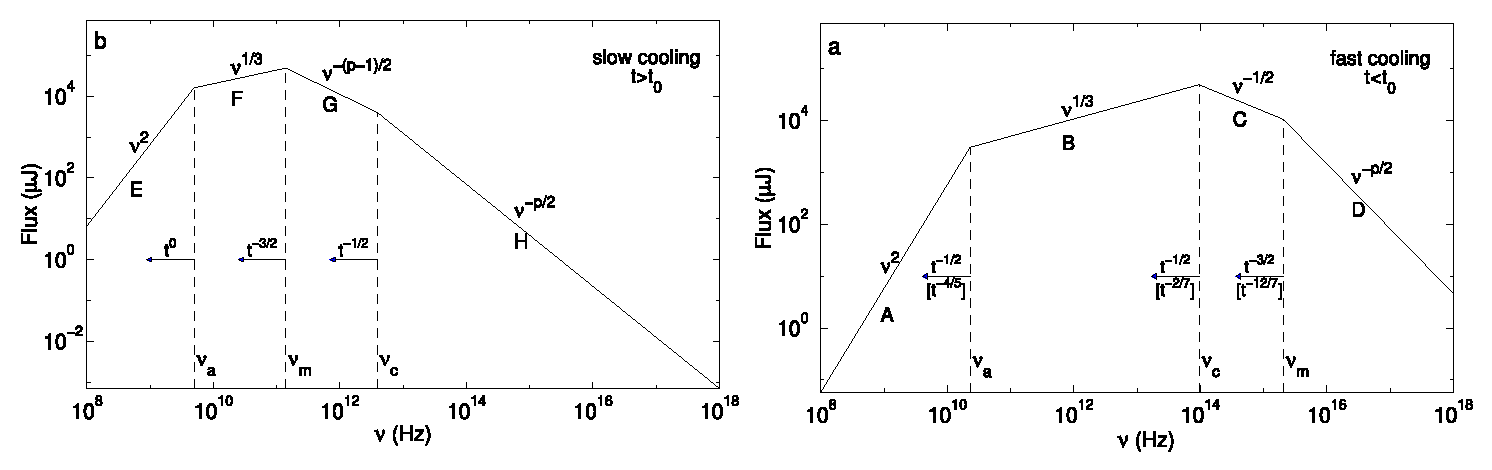
\includegraphics[height=4.8cm]{figures/sari97_flat.pdf}
            }};
        }
    \end{tikzpicture}
\end{frame}